\documentclass[portugues]{sobraep}

\titulo{MOTOR DE PASSO HÍBRIDO}

\title{HYBRID STEPPER MOTOR}


\author{Callebe S. Barbosa$^{1}$, Rafael C. Bonotto$^{2}$, Raphael H. Machado$^{3}$, Victor Emanuel S. Barbosa$^{4}$\\
	\normalsize e-mail: $^{4}$victorbarbosa@alunos.utfpr.edu.br, $^{2}$bonotto@alunos.utfpr.edu.br, @alunos.utfpr.edu.br, @alunos.utfpr.edu.br
}

\begin{document}

\maketitle

\begin{resumo}
	O objetivo deste documento é descrever o princípio de funcionamento, características construtivas, modelo matemático da motor de passo híbrido, além de mostrar algumas aplicações.
\end{resumo}

\begin{palavraschave}
	Elétrica, Máquinas, Máquinas elétricas, Motor de passo híbrido, Motor.
\end{palavraschave}

\englishtitle

\begin{abstract}
	The purpose of this document is to describe the principle of operation, construction characteristics, mathematical model of hybrid stepper motor, and show some applications.
\end{abstract}

\begin{keywords}
	Electrical, Machinery, Electrical equipment, Hybrid stepper motor, Motor.
\end{keywords}

%\newpage
\section*{NOMENCLATURAS E SIGLAS}

\symbolnomenclature{HSM}{\textit{Hybrid Stepper Motor}, Motor de passo híbrido}
\symbolnomenclature{VRM}{\textit{Variable Reluctance Motor}, Motor de relutância variável}
\symbolnomenclature{PMM}{\textit{Permanent Magnet Motor}, Motor de imã permanente}

%~~~~~~~~~~~~~~~~~~~~~~~~~~~~~~~~~~~~~~~~
% Seções
%~~~~~~~~~~~~~~~~~~~~~~~~~~~~~~~~~~~~~~~~

% Introdução
\section{INTRODUÇÃO}
	
	Os motores de passo híbrido, ou \textit{Hybrid Stepper Motor} (da sigla \textbf{HSM}) como são citados na literatura, são comumente utilizados em aplicações que demandam de alta precisão em motores de corrente contínua \cite{ieeeRusso}.
	
	O HSM, como será referido neste trabalho, combina as vantagens do motor de relutância variável (\textit{Variable Reluctance Motor}, da sigla \textbf{VRM}) e do motor de imã permanente (\textit{Permanent Magnet Motor}, da sigla \textbf{PMM}). 
	
	Como em outros motores elétricos, o motor de passo híbrido é composto por um estator e um rotor. Entretanto, as características do HSM compõem as funcionalidades principais dos dois motores, VRM e PMM, que o tornam bastante preciso e eficiente. Devido a esta particularidade, o motor em questão é denominado de \textbf{híbrido}.
	
	Um exemplo de um motor de passo híbrido simples é apresentado na Fig. \ref{HSMgrafico}.
	
	\begin{figure}
		\centering
		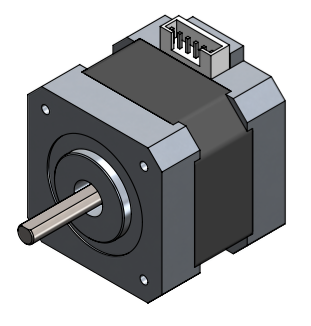
\includegraphics[width=3cm]{Images/HSMmodel.png}
		\caption{Motor de passo híbrido 17HS3001-20B (RP One Labs)}
		\label{HSMgrafico}
	\end{figure} 
	
	As características construtivas, princípio de funcionamento e acionamento do motor serão apresentadas posteriormente, no decorrer deste trabalho. 

\section{Princípio de funcionamento de um HSM}
Como explanado anteriormente, o motor de passo híbrido congrega características do motor de passo de ímã permanente e o motor de passo de relutância variável. Para entender como o motor de passo híbrido funciona, primeiramente irá ser mostrado brevemente o princípio de funcionamento destes dois outros tipos de motores de passo ora citados, bem como o que são motores de passo, por fim será explicado o funcionamento do motor de passo híbrido em função como um motor aperfeiçoado dos outros dois motores de passo, a fim da explicação se tornar mais familiarizada para o leitor.  

	\subsection{Motor de passo}
	São máquinas elétricas que consistem em um estator com enrolamentos de excitação e um rotor magnético com saliências. Neles o conjugado é produzido pela tendência do rotor a se alinhar com a onda de fluxo produzida pelo estator, de modo a maximizar os fluxos concatenados que resultam da aplicação de uma dada corrente no estator. No motor de passo as fases dos enrolamentos do estator são excitadas sequencialmente, fazendo o rotor girar na forma de uma sequência de passos, com ângulos definidos a cada passo, devido à tendência de alinhamento do rotor com a onda de fluxo do estator. \cite{Fitz} As principais características dos motores de passo são: \cite{MoonsHSM} 
	
	\begin{itemize}
		\item \textbf{Inexistência de escovas:} não necessitam de escovas, reduzindo a maioria das falhas comumente encontradas nos outros motores elétricos, como faiscamento e perdas ôhmicas no rotor e escovas.
		\item \textbf{Independência da carga:} giram com uma dada velocidade independentemente da carga, desde que tal carga não exceda as característica de torque do motor.
		\item \textbf{Menos sensores} se movem com incrementos quantificáveis, desde que com torque especificado, podendo ter conhecimento da posição do eixo.
		\item \textbf{Posição de repouso:} é possível manter o eixo estacionário, desde que seu torque seja respeitado. 
	\end{itemize}
	
	\subsection{Características construtivas gerais do HSM}
	
	Conforme citado anteriormente, o HSM contêm características importantes do VRM e do PMM, o que justifica a denominação 'híbrido'. O estator de um HSM é exatamente um estator do PMM, enquanto que o rotor de um HSM é um rotor do VRM magnetizado.
	
	Como forma de visualizar melhor as duas partes do motor, a Fig. \ref{HSMreal} apresenta o estator e o rotor de um HSM genérico aberto. As especificações deste motor são bem semelhantes ao motor apresentado na Fig. \ref{HSMgrafico}.
	
	\begin{figure}[!h]
		\centering
		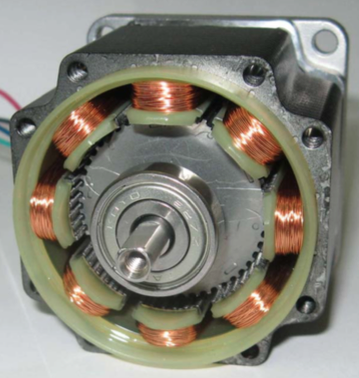
\includegraphics[scale=.45]{Images/hsmreal1.png}
		\caption{Principais partes de um HSM genérico - Visão geral \cite{ieeeRusso}}
		\label{HSMreal}
	\end{figure} 
	
	O estator de um motor de passo híbrido é composto por um dado número de polos magnéticos relacionados com o número de enrolamentos nele, exatamente como em um PMM. Essa característica é herdada dos motores de imã permanente. No PMM, admite-se que para melhorar a resolução de passo, basta adicionar mais enrolamentos ou adicionar mais pares de polos no rotor, através do campo magnético produzido nos enrolamentos deste estator. 
	
	O rotor de um motor de passo híbrido é cuidadosamente seccionado, criando pequenas lacunas chamadas dentes (\textit{teeth}) para gerar uma compensação (\textit{offset}) com relação ao estator para o rotor executar a rotação. É importante citar que o rotor de um HSM é magnetizado, diferentemente do rotor de um VRM.
	
	\begin{figure}[!h]
		\centering
		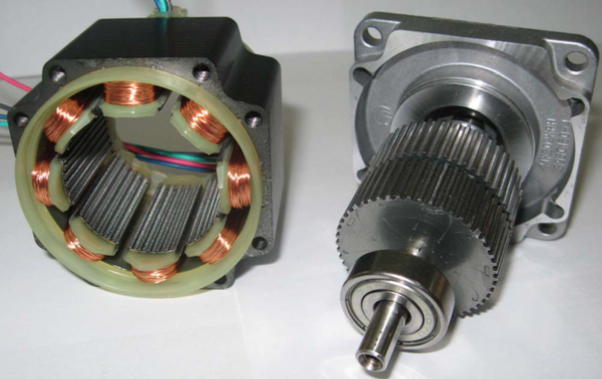
\includegraphics[scale=.4]{Images/hsmreal2.png}
		\caption{Estator (à esquerda) e rotor (à direita) de um HSM genérico \cite{ieeeRusso}}
		\label{HSMestatorrotor}
	\end{figure} 
	
	Verifica-se pela Fig. \ref{HSMestatorrotor} que o estator também é seccionado com alguns dentes. A razão do estator também possuir esses dentes é com o propósito de fazer o motor operar, o que será explanado a seguir.
	
	\subsection{Funcionamento do motor de passo híbrido}
	
	%PARTE QUE O BONOTTO SE RESPONSABILIZA EM TERMINAR :)

\section{Características construtivas}

	%Rotor é um material não magnetico.

\section{Comparação entre os motores de passo}

\begin{table*}[!h]
\centering
\caption{Comparação entre os motores de passo VRM, PMM e HSM (Microchip WebSeminars, 2012)}
\label{my-label}
\begin{tabular}{|c|c|c|c|}
\hline
\textit{Característica} & \textbf{PMM} & \textbf{VRM} & \textbf{HSM} \\ \hline
\textit{\begin{tabular}[c]{@{}c@{}}Custo de \\ produção\end{tabular}} & Barato & Moderado & Muito Caro \\ \hline
\textit{Design} & \begin{tabular}[c]{@{}c@{}}Moderadamente \\ Complexo\end{tabular} & Simples & Complexo \\ \hline
\textit{Resolução} & 30º-3º/passo & \multicolumn{2}{c|}{1,8º/passo ou menor} \\ \hline
\textit{Ruído} & Não há & \begin{tabular}[c]{@{}c@{}}Há ruido independente\\ do tipo de excitação\end{tabular} & Não há \\ \hline
\textit{Passo} & \begin{tabular}[c]{@{}c@{}}Passo cheio, meio passo\\ e micro-passo\end{tabular} & \begin{tabular}[c]{@{}c@{}}Normalmente opera em\\ passo cheio\end{tabular} & \begin{tabular}[c]{@{}c@{}}Passo cheio, meio passo\\ e micro-passo\end{tabular} \\ \hline
\end{tabular}
\end{table*}

\section{Modelo matemático}

\section{Exemplos de aplicações}
Os motores de passo, inclusive o de passo híbrido, são amplamente utilizados em sistemas de controle digital, motores de alimentação de papel e posicionamento da cabeça em unidade de discos, entre outras. Por não terem enrolamentos no rotor, eles têm boa densidade de potência, pois não há necessidade de grande dissipação de calor do rotor, e também têm grande aplicação em aplicações onde é necessário realizar movimentos precisos e ter conhecimento da posição do rotor sem necessidade de realimentação com sensores. O motor de passo híbrido ainda tem melhores características de conjugado, velocidade e precisão nos passos. \cite{Fitz}

\section{CONCLUSÕES}



\bibliographystyle{bib_sobraep}
\bibliography{referencias_sobraep}

\end{document}